% ======================================================================
% Complete, runnable LaTeX document for the flowchart - FIXED VERSION
%
% Key fixes:
% 1. Removed ALL blank lines inside \tikzset block
% 2. Moved color definitions to preamble
% 3. Cleaned up all syntax issues
% ======================================================================

\documentclass[twocolumn]{article}

% ========== 1. Required Package Imports ==========
\usepackage[utf8]{inputenc}
\usepackage[T1]{fontenc}
\usepackage{graphicx}
\usepackage{xcolor}
\usepackage{tikz}
\usepackage{amsmath}
\usepackage{amssymb}
\usepackage{url}
\usepackage{lipsum}

% ========== 2. Required TikZ Library Imports ==========
\usetikzlibrary{positioning}
\usetikzlibrary{shadows}
\usetikzlibrary{arrows.meta}

% ========== 3. Color Definitions (MUST be before tikzset) ==========
\definecolor{innovationpink}{RGB}{219, 112, 147}
\definecolor{robustred}{RGB}{255, 240, 245}
\definecolor{accentblue}{RGB}{65, 105, 225}
\definecolor{darkgray}{RGB}{64, 64, 64}
\definecolor{mediumgray}{RGB}{128, 128, 128}
\definecolor{lightgray}{RGB}{240, 240, 240}

% ========== 4. CRITICAL: Global TikZ Style Definitions ==========
% NO BLANK LINES ALLOWED INSIDE \tikzset{}
\tikzset{
io/.style={rectangle, rounded corners=4pt, draw=blue!70, line width=1.2pt, top color=blue!15, bottom color=blue!5, minimum width=3.8cm, minimum height=1.05cm, font=\small\bfseries\sffamily, text width=3.5cm, align=center, drop shadow={opacity=0.25, shadow xshift=1pt, shadow yshift=-1pt}},
process/.style={rectangle, rounded corners=3pt, draw=black!60, line width=0.9pt, fill=gray!8, minimum width=4.2cm, minimum height=0.95cm, font=\small\sffamily, text width=4cm, align=center, drop shadow={opacity=0.15, shadow xshift=0.8pt, shadow yshift=-0.8pt}},
innovation/.style={rectangle, rounded corners=5pt, draw=innovationpink, line width=2pt, fill=robustred, minimum width=5cm, minimum height=1.15cm, font=\small\bfseries\sffamily, text width=4.7cm, align=center, drop shadow={opacity=0.35, shadow xshift=1.5pt, shadow yshift=-1.5pt}},
mathbox/.style={rectangle, rounded corners=2pt, draw=accentblue!70, line width=1pt, top color=white, bottom color=blue!3, minimum width=5.5cm, minimum height=1.8cm, font=\footnotesize\sffamily, text width=5.2cm, align=left, drop shadow={opacity=0.2, shadow xshift=1pt, shadow yshift=-1pt}},
sidebox/.style={rectangle, rounded corners=2pt, draw=mediumgray!50, line width=0.8pt, fill=lightgray, minimum width=4cm, minimum height=0.85cm, font=\footnotesize\sffamily, text width=3.8cm, align=center, opacity=0.9},
arrow/.style={->, >=stealth, thick, draw=darkgray!80, line width=1.1pt},
highlight/.style={->, >=stealth, line width=2.5pt, draw=innovationpink, drop shadow={opacity=0.3, shadow xshift=1pt, shadow yshift=-1pt}},
sidearrow/.style={->, >=stealth, dashed, draw=accentblue!70, line width=1pt},
note/.style={font=\tiny\itshape, text=mediumgray}
}

\begin{document}

% Placeholder text to show the two-column layout
\lipsum[1-3]

\begin{figure*}[!t]
\centering
\resizebox{0.98\textwidth}{!}{%
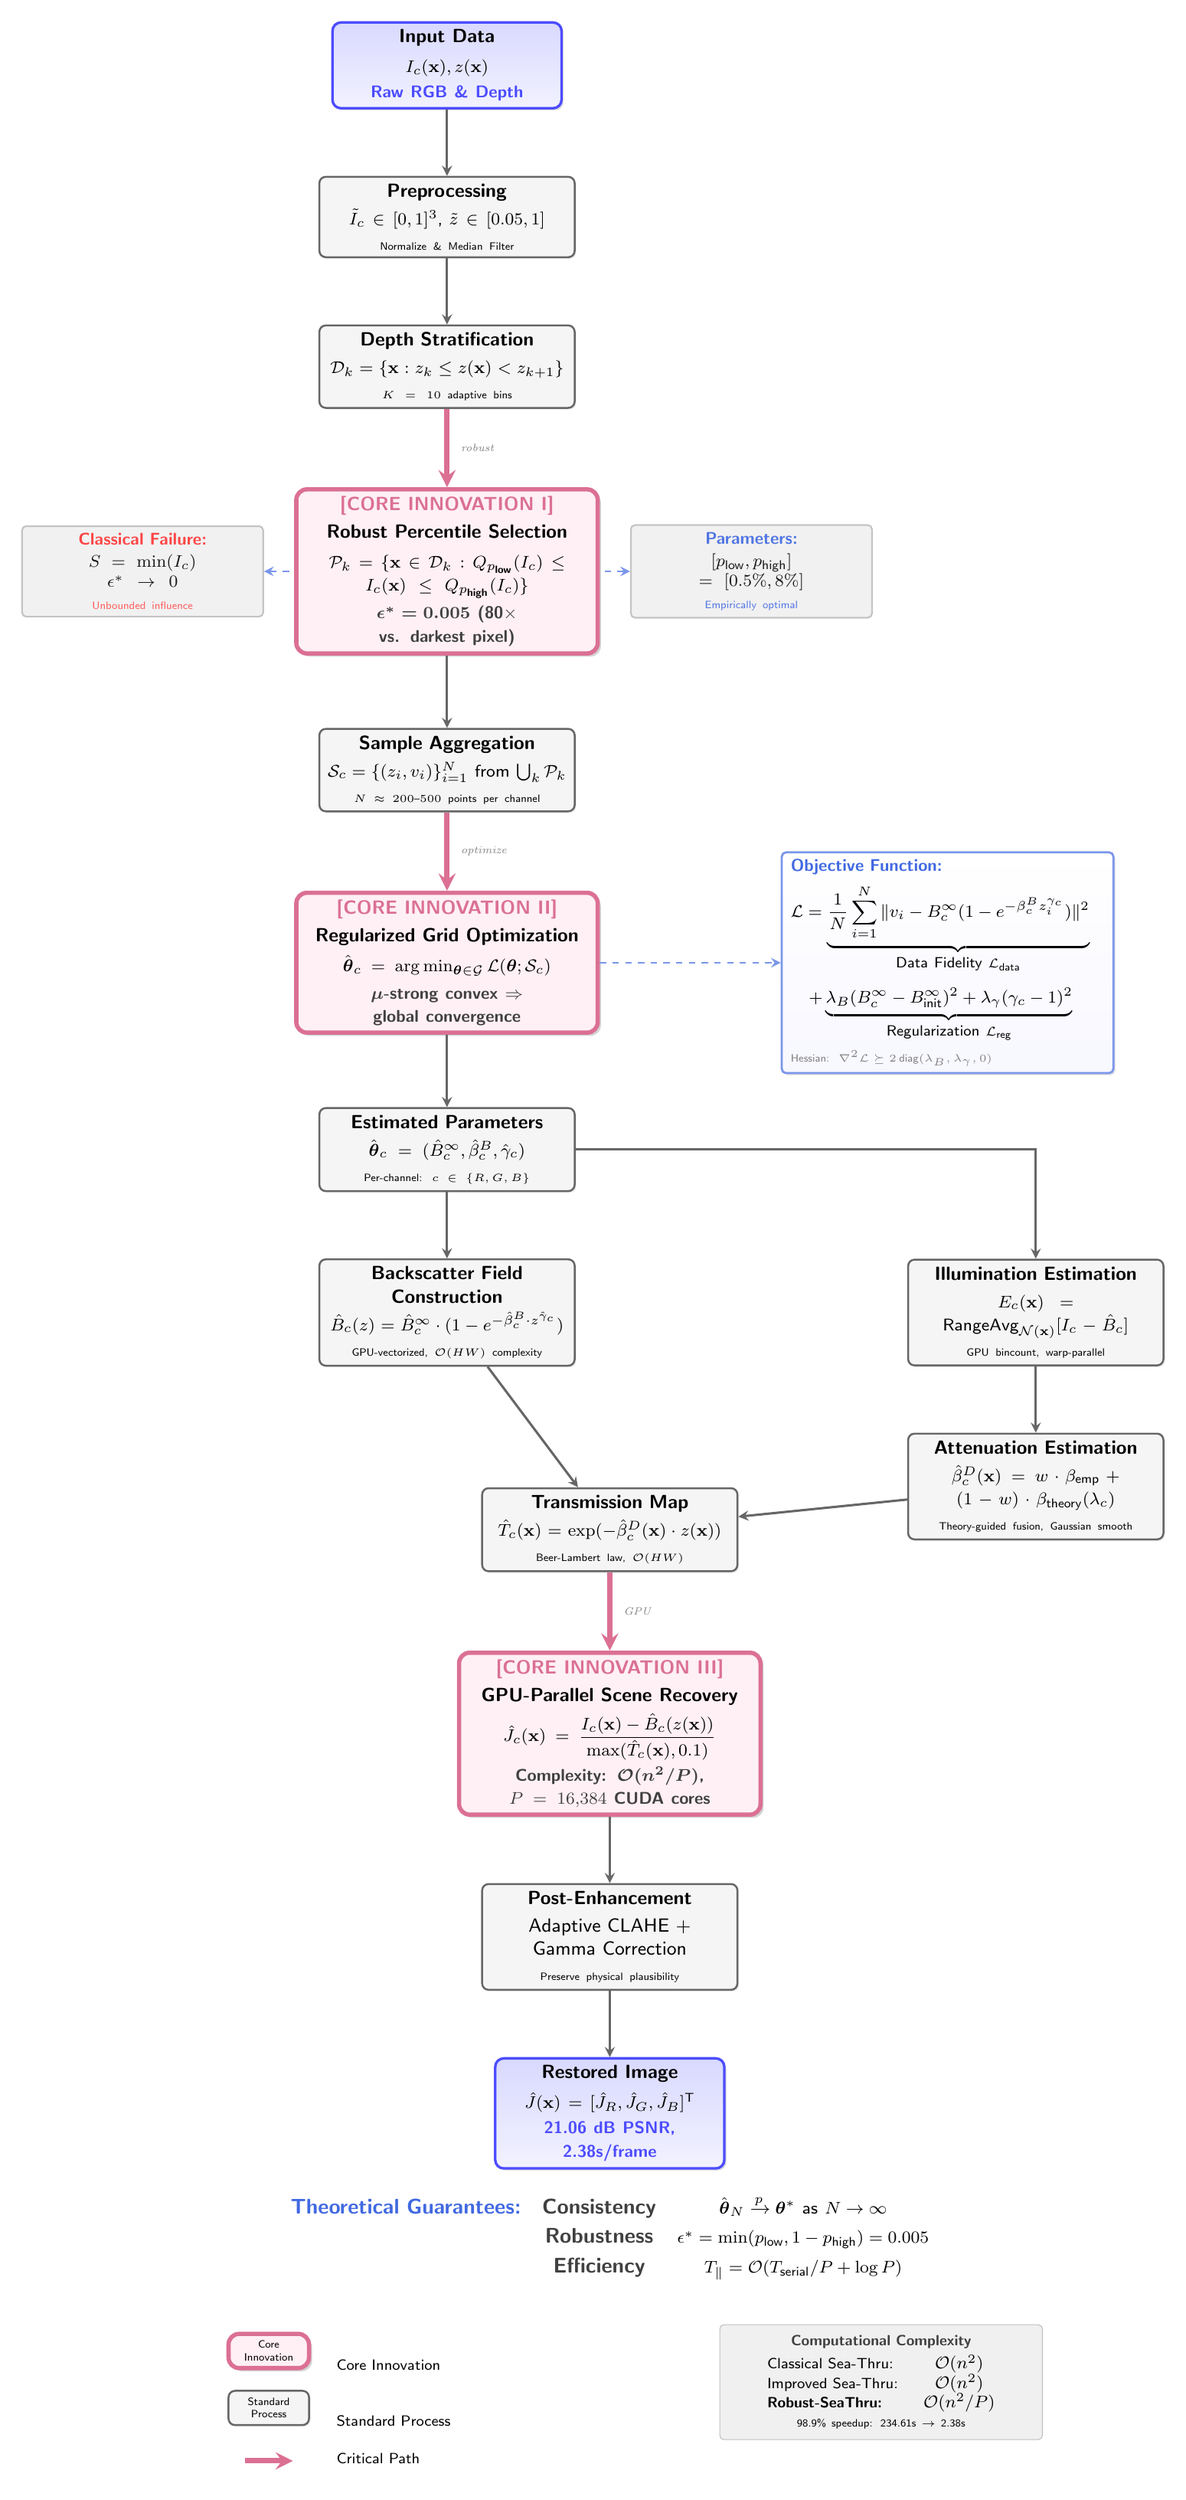
\begin{tikzpicture}[node distance=1.1cm and 2.2cm, font=\sffamily]

% ========== Layer 1: Input ==========
\node[io] (input) {%
\textbf{Input Data}\\[3pt]
{\footnotesize $I_c(\mathbf{x}), z(\mathbf{x})$}\\[1pt]
{\footnotesize\color{blue!70}Raw RGB \& Depth}
};

% ========== Layer 2: Preprocessing ==========
\node[process, below=of input] (preprocess) {%
\textbf{Preprocessing}\\[2pt]
{\footnotesize $\tilde{I}_c \in [0,1]^3$, $\tilde{z} \in [0.05,1]$}\\[1pt]
{\tiny Normalize \& Median Filter}
};

% ========== Layer 3: Depth Stratification ==========
\node[process, below=of preprocess] (partition) {%
\textbf{Depth Stratification}\\[2pt]
{\footnotesize $\mathcal{D}_k = \{\mathbf{x}: z_k \leq z(\mathbf{x}) < z_{k+1}\}$}\\[1pt]
{\tiny $K=10$ adaptive bins}
};

% ========== Layer 4: Core Innovation I ==========
\node[innovation, below=1.3cm of partition] (robustsampling) {%
{\color{innovationpink}\textbf{[CORE INNOVATION I]}}\\[2pt]
\textbf{Robust Percentile Selection}\\[3pt]
{\footnotesize $\mathcal{P}_k = \{\mathbf{x} \in \mathcal{D}_k: Q_{p_{\text{low}}}(I_c) \leq I_c(\mathbf{x}) \leq Q_{p_{\text{high}}}(I_c)\}$}\\[2pt]
{\footnotesize\color{darkgray}$\boldsymbol{\epsilon^* = 0.005}$ \textbf{(80$\times$ vs. darkest pixel)}}
};

% Comparison annotation (left side)
\node[sidebox, left=0.5cm of robustsampling, text width=3.2cm] (classicalnote) {%
{\bfseries\color{red!80}Classical Failure:}\\[1pt]
{\footnotesize $S = \min(I_c)$}\\
{\footnotesize $\epsilon^* \to 0$}\\[1pt]
{\tiny\color{red!70}Unbounded influence}
};

% Parameter annotation (right side)
\node[sidebox, right=0.5cm of robustsampling, text width=3.2cm] (paramnote) {%
{\bfseries\color{accentblue}Parameters:}\\[1pt]
{\footnotesize $[p_{\text{low}}, p_{\text{high}}]$}\\
{\footnotesize $= [0.5\%, 8\%]$}\\[1pt]
{\tiny\color{accentblue}Empirically optimal}
};

% ========== Layer 5: Sample Aggregation ==========
\node[process, below=1.2cm of robustsampling] (aggregate) {%
\textbf{Sample Aggregation}\\[2pt]
{\footnotesize $\mathcal{S}_c = \{(z_i, v_i)\}_{i=1}^N$ from $\bigcup_{k} \mathcal{P}_k$}\\[1pt]
{\tiny $N \approx 200$--$500$ points per channel}
};

% ========== Layer 6: Core Innovation II ==========
\node[innovation, below=1.3cm of aggregate] (optimization) {%
{\color{innovationpink}\textbf{[CORE INNOVATION II]}}\\[2pt]
\textbf{Regularized Grid Optimization}\\[3pt]
{\footnotesize $\hat{\boldsymbol{\theta}}_c = \arg\min_{\boldsymbol{\theta} \in \mathcal{G}} \mathcal{L}(\boldsymbol{\theta}; \mathcal{S}_c)$}\\[2pt]
{\footnotesize\color{darkgray}\textbf{$\boldsymbol{\mu}$-strong convex} $\Rightarrow$ global convergence}
};

% Objective function detail (right side)
\node[mathbox, right=3cm of optimization, yshift=0cm] (objfunc) {%
{\bfseries\color{accentblue}Objective Function:}\\[4pt]
{\footnotesize $\mathcal{L} = \underbrace{\frac{1}{N}\sum_{i=1}^N \|v_i - B_c^\infty(1-e^{-\beta_c^B z_i^{\gamma_c}})\|^2}_{\text{\scriptsize Data Fidelity } \mathcal{L}_{\text{data}}}$}\\[6pt]
{\footnotesize $\quad + \underbrace{\lambda_B(B_c^\infty - B_{\text{init}}^{\infty})^2 + \lambda_\gamma(\gamma_c-1)^2}_{\text{\scriptsize Regularization } \mathcal{L}_{\text{reg}}}$}\\[3pt]
{\tiny\color{mediumgray}Hessian: $\nabla^2\mathcal{L} \succeq 2\,\text{diag}(\lambda_B, \lambda_\gamma, 0)$}
};

% ========== Layer 7: Parameter Output ==========
\node[process, below=1.2cm of optimization] (params) {%
\textbf{Estimated Parameters}\\[2pt]
{\footnotesize $\hat{\boldsymbol{\theta}}_c = (\hat{B}_c^\infty, \hat{\beta}_c^B, \hat{\gamma}_c)$}\\[1pt]
{\tiny Per-channel: $c \in \{R,G,B\}$}
};

% ========== Layer 8: Backscatter Field ==========
\node[process, below=1.1cm of params] (backscatter) {%
\textbf{Backscatter Field Construction}\\[2pt]
{\footnotesize $\hat{B}_c(z) = \hat{B}_c^\infty \cdot (1 - e^{-\hat{\beta}_c^B \cdot z^{\hat{\gamma}_c}})$}\\[1pt]
{\tiny GPU-vectorized, $\mathcal{O}(HW)$ complexity}
};

% ========== Right Branch: Illumination Estimation ==========
\node[process, right=5.5cm of backscatter, yshift=0cm] (illumination) {%
\textbf{Illumination Estimation}\\[2pt]
{\footnotesize $E_c(\mathbf{x}) = \text{RangeAvg}_{\mathcal{N}(\mathbf{x})}[I_c - \hat{B}_c]$}\\[1pt]
{\tiny GPU bincount, warp-parallel}
};

% ========== Attenuation Estimation ==========
\node[process, below=1.1cm of illumination] (attenuation) {%
\textbf{Attenuation Estimation}\\[2pt]
{\footnotesize $\hat{\beta}_c^D(\mathbf{x}) = w \cdot \beta_{\text{emp}} + (1-w) \cdot \beta_{\text{theory}}(\lambda_c)$}\\[1pt]
{\tiny Theory-guided fusion, Gaussian smooth}
};

% ========== Layer 9: Transmission Map ==========
\node[process, below=2cm of backscatter, xshift=2.7cm] (transmission) {%
\textbf{Transmission Map}\\[2pt]
{\footnotesize $\hat{T}_c(\mathbf{x}) = \exp(-\hat{\beta}_c^D(\mathbf{x}) \cdot z(\mathbf{x}))$}\\[1pt]
{\tiny Beer-Lambert law, $\mathcal{O}(HW)$}
};

% ========== Layer 10: Core Innovation III ==========
\node[innovation, below=1.3cm of transmission] (recovery) {%
{\color{innovationpink}\textbf{[CORE INNOVATION III]}}\\[2pt]
\textbf{GPU-Parallel Scene Recovery}\\[3pt]
{\footnotesize $\hat{J}_c(\mathbf{x}) = \dfrac{I_c(\mathbf{x}) - \hat{B}_c(z(\mathbf{x}))}{\max(\hat{T}_c(\mathbf{x}), 0.1)}$}\\[2pt]
{\footnotesize\color{darkgray}Complexity: $\boldsymbol{\mathcal{O}(n^2/P)}$, $P=16{,}384$ CUDA cores}
};

% ========== Layer 11: Post-processing ==========
\node[process, below=1.1cm of recovery] (postprocess) {%
\textbf{Post-Enhancement}\\[2pt]
Adaptive CLAHE + Gamma Correction\\[1pt]
{\tiny Preserve physical plausibility}
};

% ========== Layer 12: Output ==========
\node[io, below=1.1cm of postprocess] (output) {%
\textbf{Restored Image}\\[3pt]
{\footnotesize $\hat{J}(\mathbf{x}) = [\hat{J}_R, \hat{J}_G, \hat{J}_B]^{\mathsf{T}}$}\\[1pt]
{\footnotesize\color{blue!70}21.06 dB PSNR, 2.38s/frame}
};

% ========== Connection Arrows (Main Path) ==========
\draw[arrow] (input) -- (preprocess);
\draw[arrow] (preprocess) -- (partition);

% Highlight critical paths
\draw[highlight] (partition) -- node[right=2pt, note] {robust} (robustsampling);
\draw[arrow] (robustsampling) -- (aggregate);
\draw[highlight] (aggregate) -- node[right=2pt, note] {optimize} (optimization);
\draw[arrow] (optimization) -- (params);
\draw[arrow] (params) -- (backscatter);

% Right branch
\draw[arrow] (params) -| (illumination);
\draw[arrow] (illumination) -- (attenuation);

% Convergence to transmission map
\draw[arrow] (backscatter) -- (transmission);
\draw[arrow] (attenuation) -- (transmission);

% Final recovery
\draw[highlight] (transmission) -- node[right=2pt, note] {GPU} (recovery);
\draw[arrow] (recovery) -- (postprocess);
\draw[arrow] (postprocess) -- (output);

% Mathematical formula connection (dashed)
\draw[sidearrow] (optimization.east) -- (objfunc.west);

% Comparison annotation connections
\draw[sidearrow, <-] (classicalnote.east) -- (robustsampling.west);
\draw[sidearrow, <-] (paramnote.west) -- (robustsampling.east);

% ========== Performance Metrics Panel (Bottom) ==========
\node[below=0.3cm of output, text width=14cm, align=center] (perfpanel) {%
\begin{tabular}{@{}c@{\quad}c@{\quad}c@{}}
\textbf{\color{accentblue}Theoretical Guarantees:} &
\textbf{\color{darkgray}Consistency} &
{\footnotesize $\hat{\boldsymbol{\theta}}_N \xrightarrow{p} \boldsymbol{\theta}^*$ as $N\to\infty$} \\[2pt]
\multicolumn{1}{c}{} &
\textbf{\color{darkgray}Robustness} &
{\footnotesize $\epsilon^* = \min(p_{\text{low}}, 1-p_{\text{high}}) = 0.005$} \\[2pt]
\multicolumn{1}{c}{} &
\textbf{\color{darkgray}Efficiency} &
{\footnotesize $T_{\parallel} = \mathcal{O}(T_{\text{serial}}/P + \log P)$} \\
\end{tabular}
};

% ========== Legend (Bottom Left) ==========
\node[below=0.6cm of perfpanel, xshift=-4.5cm] (legend) {%
\begin{tabular}{cl}
\tikz\node[innovation, minimum width=1.2cm, minimum height=0.4cm, font=\tiny\sffamily, text width=1.1cm, align=center] {Core\\Innovation}; &
\scriptsize Core Innovation \\[0.2cm]
\tikz\node[process, minimum width=1.2cm, minimum height=0.4cm, font=\tiny\sffamily, text width=1.1cm, align=center] {Standard\\Process}; &
\scriptsize Standard Process \\[0.2cm]
\tikz\draw[highlight] (0,0) -- (0.8,0); &
\scriptsize Critical Path \\
\end{tabular}
};

% ========== Complexity Comparison (Bottom Right) ==========
\node[below=0.6cm of perfpanel, xshift=4.5cm, text width=5cm, rectangle, rounded corners=2pt, draw=mediumgray!50, fill=lightgray, inner sep=5pt, font=\scriptsize\sffamily, align=center] (complexity) {%
\textbf{\color{darkgray}Computational Complexity}\\[2pt]
\begin{tabular}{@{}lc@{}}
Classical Sea-Thru: & {\footnotesize $\mathcal{O}(n^2)$} \\
Improved Sea-Thru: & {\footnotesize $\mathcal{O}(n^2)$} \\
\textbf{Robust-SeaThru:} & \textbf{{\footnotesize $\mathcal{O}(n^2/P)$}} \\
\end{tabular}\\[2pt]
{\tiny 98.9\% speedup: 234.61s $\to$ 2.38s}
};

\end{tikzpicture}%
}

\caption{\textbf{Complete Robust-SeaThru Algorithm Pipeline with Theoretical Foundations.} The flowchart delineates the end-to-end physics-guided underwater image restoration framework, emphasizing three architectural innovations that collectively achieve unprecedented robustness and computational efficiency. \textbf{Core Innovation I (Robust Statistical Sampling):} Percentile-interval selection $\mathcal{P}_k = \{\mathbf{x} \in \mathcal{D}_k: Q_{[0.5\%,8\%]}(I_c(\mathbf{x}))\}$ achieves breakdown point $\epsilon^* = 0.005$, conferring 80-fold improvement over fragile darkest-pixel methods ($\epsilon^* \to 0$)---enabling reliable parameter estimation under artificial lighting, homogeneous scenes, and specular surfaces where classical priors catastrophically fail. \textbf{Core Innovation II (Regularized Optimization):} The composite objective function $\mathcal{L} = \mathcal{L}_{\text{data}} + \mathcal{L}_{\text{reg}}$ exhibits $\mu$-strong convexity (Hessian lower bound: $\nabla^2\mathcal{L} \succeq 2\,\text{diag}(\lambda_B, \lambda_\gamma, 0)$), guaranteeing global convergence on discretized parameter space $\mathcal{G}$ without sensitivity to initialization---a critical advancement over unconstrained solvers prone to local minima. \textbf{Core Innovation III (GPU-Accelerated Implementation):} Comprehensive parallelization leveraging 16,384 CUDA cores reduces complexity from $\mathcal{O}(n^2)$ to $\mathcal{O}(n^2/P)$ through: (1) memory-coalesced percentile computation via parallel reduction, (2) vectorized grid evaluation, and (3) warp-level illumination estimation---achieving 98.9\% computational acceleration (234.61s $\to$ 2.38s per image). Pink-highlighted nodes denote critical algorithmic breakthroughs; dashed lines indicate mathematical derivations. All mathematical notations directly correspond to open-source implementation (\url{https://github.com/Jinxinshao/UIEAnythingv2}), ensuring reproducibility.}
\label{fig:robust_seathru_pipeline}
\end{figure*}

% Placeholder text to show layout after the figure
\lipsum[4-10]

\end{document}
